\documentclass{homeworg}
\usepackage{amsmath}

\title{Travail 4 - Circuits RC}
\author{Wats Raphaël}

\begin{document}
\maketitle

\section{Schéma du circuit}
    \begin{center}
        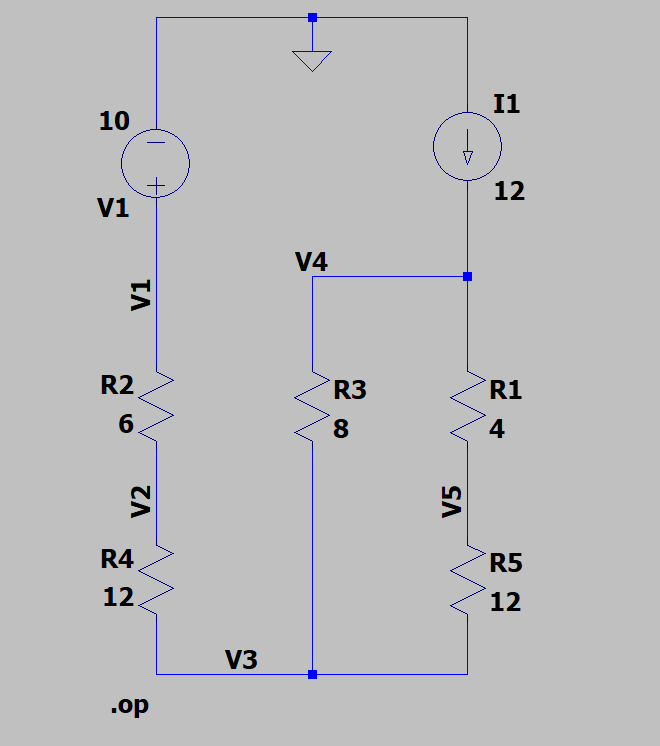
\includegraphics[scale=0.35]{Shematic.png}
    \end{center}

\newpage
\section{Le calcul de la condition initiale}
    \begin{center}
        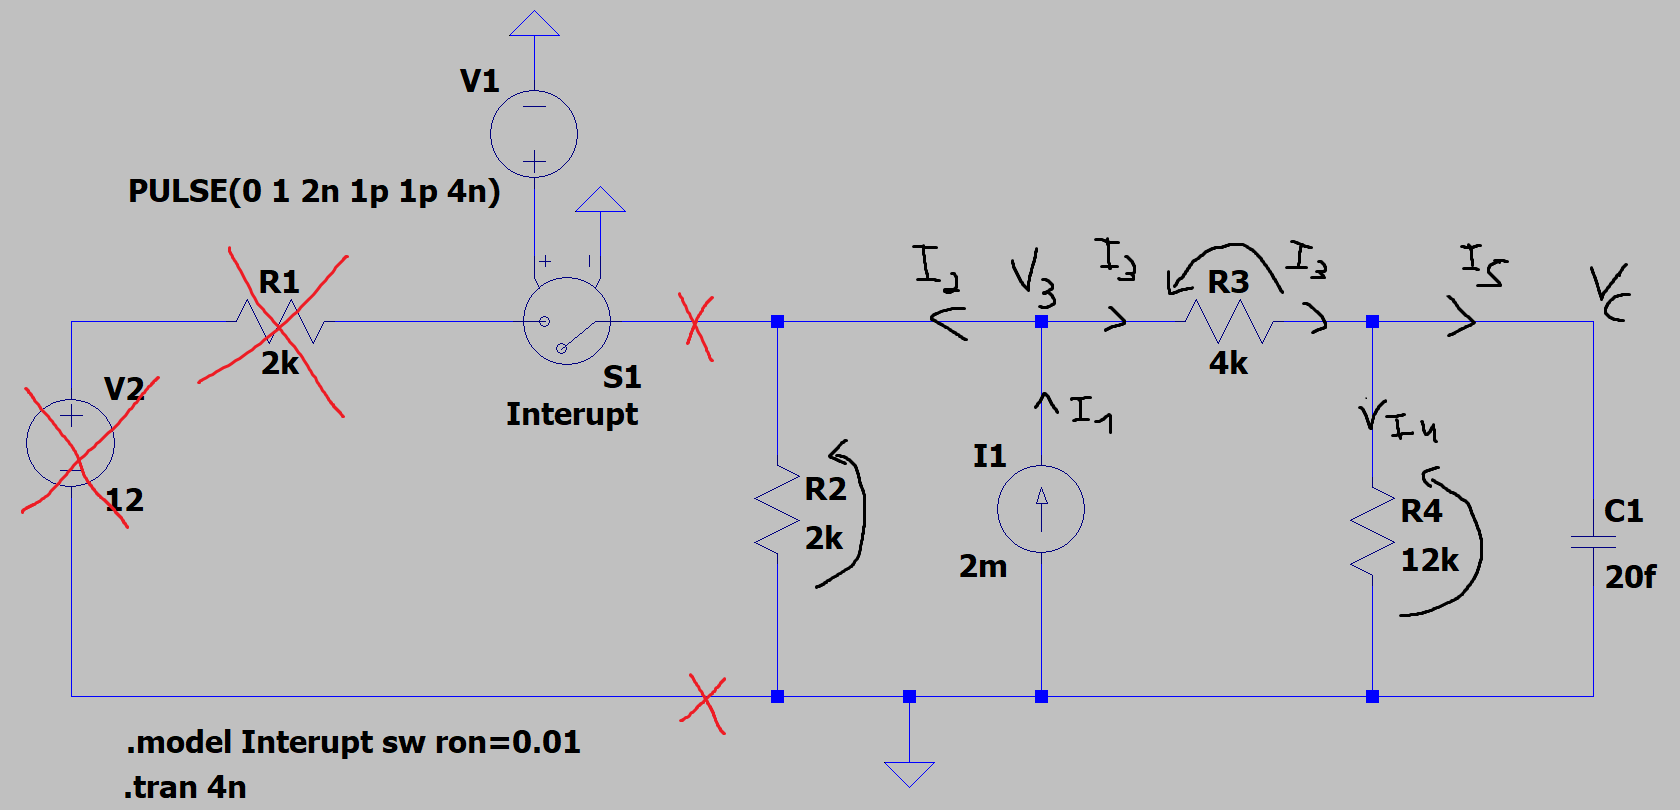
\includegraphics[scale=0.35]{Vinit.png}
    \end{center}
    Comme la capacité est entièrement chargée, le courant $I_5$ dans la capacité est nul.
    \begin{align}
        I_1 = I_2 + I_3\\
        I_3 = I_4 + I_5\\
        I_5 = 0\\
        I_3 = I_4\\
    \end{align}
    En exprimant $V_3$ en terme de $V_c$ on peut résoudre le noeud de $V_3$
    \begin{align}
        I_2 = V_3 / R_2\\
        I_3 = (V_3 - V_c) / R_3\\
        I_3 = V_c / R_4\\
        (V_3 - V_c) / R_3 = V_c / R_4\\
        V_3 = (V_c * R_3) / R_4 + V_c = (V_c * 4000) / 12000 + V_c\\
        V_3 = 4V_c / 3\\
        I_2 = (4V_c / 3) / R_2 = 4V_c / 6000 = 2V_c / 3000\\
        I_1 = 2V_c / 3000 + V_c / 12000\\
        0.002 = 9V_c / 12000\\
        V_c = 8/3 = 2.67V
    \end{align}

\newpage
\section{Le calcul de la condition finale}
    \begin{center}
        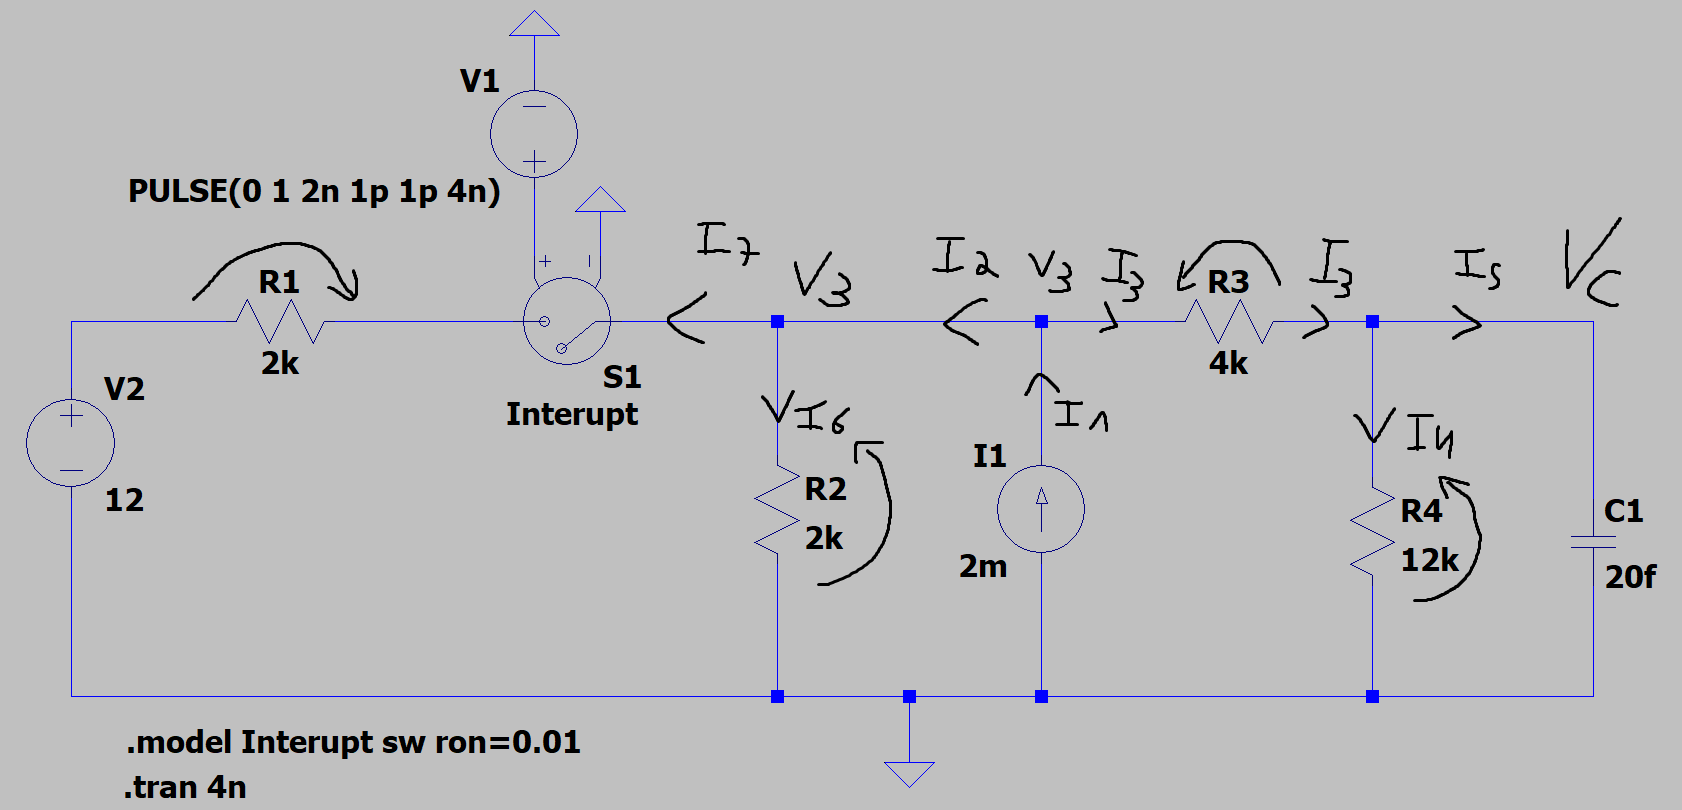
\includegraphics[scale=0.35]{Vfinal.png}
    \end{center}
    On met tout d'abord en équation les différents noeuds du circuit.\\
    Comme la capacité est entièrement chargée, le courant $I_5$ dans la capacité est nul.
    \begin{align}
        I_1 = I_2 + I_3\\
        I_2 = I_6 + I_7\\
        I_3 = I_4 + I_5\\
        I_3 = I_5
    \end{align}
    
    Exprimer le premier noeud en terme de $V_3$ et $V_c$
    \begin{align}
        I_6 = V_3 / R_2\\
        I_7 = (V_3 - V_2) / R_1\\
        I_2 = V_3 / R_2 + (V_3 - V_2) / R_1\\
        I_3 = (V_3 - V_c) / R_3\\
        I_1 = V_3 / R_2 + (V_3 - V_2) / R_1 + (V_3 - V_c) / R_3
    \end{align}
    
    Il nous reste à exprimer à présent $V_c$ en terme de $V_3$
    \begin{align}
        I_3 = (V_3 - V_c) / R_3\\
        I_3 = V_c / R_4\\
        (V_3 - V_c) / R_3 = V_c / R_4\\
        V_3 = (V_c * R_3) / R_4 + V_c = (V_c * 4000) / 12000 + V_c\\
        V_c = 3V_3 / 4
    \end{align}
    
    il n’y a plus qu’à substituer dans la relation [3.8]
    \begin{align}
        I_1 = V_3 / R_2 + (V_3 - V_2) / R_1 + (V_3 - (3V_3 / 4)) / R_3\\
        V_3 = 128/17 = 7.53V\\
        V_c = (3 * (128 / 17)) / 4 = 96/17 = 5.65V
    \end{align}

\newpage
\section{Le calcul de la constante de temps}
$\tau = R_{eq} * C$, où $R_{eq}$ est la résistance équivalent vu par la capacité $R_{eq} = ((R_1 // R_2) + R_3) // R_4 = 3529\Omega$ et C la valeur de la capacité. $\tau = 3529\Omega * 20fF = 70p$ secondes

\section{Le calcul de la tension aux bornes de la capacité}
La solution de l'équation différentielle du premier ordre pour calculer la tension aux bornes d'une capacité est:
\begin{align}
     V_c(t) = A + B e^{-t / \tau}
\end{align}

On a alors, $V_c(t=0) = 2.67V$ à la condition initial et $V_c(t=\infty)= 5.65V$ à la condition finale
\begin{align}
    V_c(0) = A + B e^{0/ \tau} = 2.67V\\
    V_c(\infty) = A + B e^{-\infty/ \tau} = 5.65V
\end{align}

Grâce à la relation [4.2] on peut exprimer B en terme de A:
\begin{align}
    V_c(0) = A + B e^{0/ \tau} = 2.67V\\
    V_c(0) = A + B e^{0} = 2.67V\\
    V_c(0) = A + B * 1 = 2.67V\\
    V_c(0) = A + B = 2.67V\\
    B = 2.67V - A
\end{align}

On obtient la valeur de A Grâce à la relation [4.3]
\begin{align}
    V_c(\infty) = A + B e^{-\infty/ \tau} = 5.65V\\
    V_C(\infty) = A + B (1 / e^{\infty/ \tau} = 5.65V\\
    V_C(\infty) = A + B * 0 = 5.65V\\
    V_C(\infty) = A = 5.65V
\end{align}

Avec la relation [4.8] on a que $A = 5.65V$ et $B = -2.98V$ on a alors la relation [4.1]
\begin{align}
    V_c(t) = 5.65 - 2.98 e^{-t / \tau}
\end{align}
On a présent déterminer la fonction permettant de connaître l'évolution de la tension aux bornes de la capacité en fonction du temps. On peut à présent vérifier grâce à la simulation !

\newpage
Pour $t = 0.05n$ secondes (on sera alors à $2.05n$ secondes sur notre simulation) on aura:
\begin{align}
    V_c(50*10^{-12}) = 5.65 - 2.98 e^{-50*10^{-12} / 70 * 10^{-12}} = 4.185V
\end{align}
\begin{center}
    \includegraphics[scale=0.45]{GraphPoint.PNG}
\end{center}

\newpage
\section{Le calcul du courant de la capacité}
    Le courant dans la capacité en fonction du temps est donné par la relation:
    \begin{align}
        I_c(t) = C V_c(t)'\\
        I_c(t) = 20 * 10^{-15} (2.98/\tau)e^{-t/\tau}
    \end{align}
    où C est égale à la valeur de la capacité et $V_c(t)'$ est la dérivée de la fonction qui donne la valeur de la tension aux bornes de la capacité en fonction du temps.
    
    Pour $t = 0.05n$ secondes (on sera alors à $2.05n$ secondes sur notre simulation) on aura:
    \begin{align}
        I_c(50*10^{-12}) = 20 * 10^{-15} (2.98/70 * 10^{-12})e^{-50*10^{-12}/70 * 10^{-12}}\\
        I_c(50*10^{-12}) = 20 * 10^{-15} (2.98/70 * 10^{-12})e^{-5/7}\\
        I_c(50*10^{-12}) = 8,51 * 10^{-4}e^{-5/7} = 4.17 * 10^{-4}A
    \end{align}
    \begin{center}
        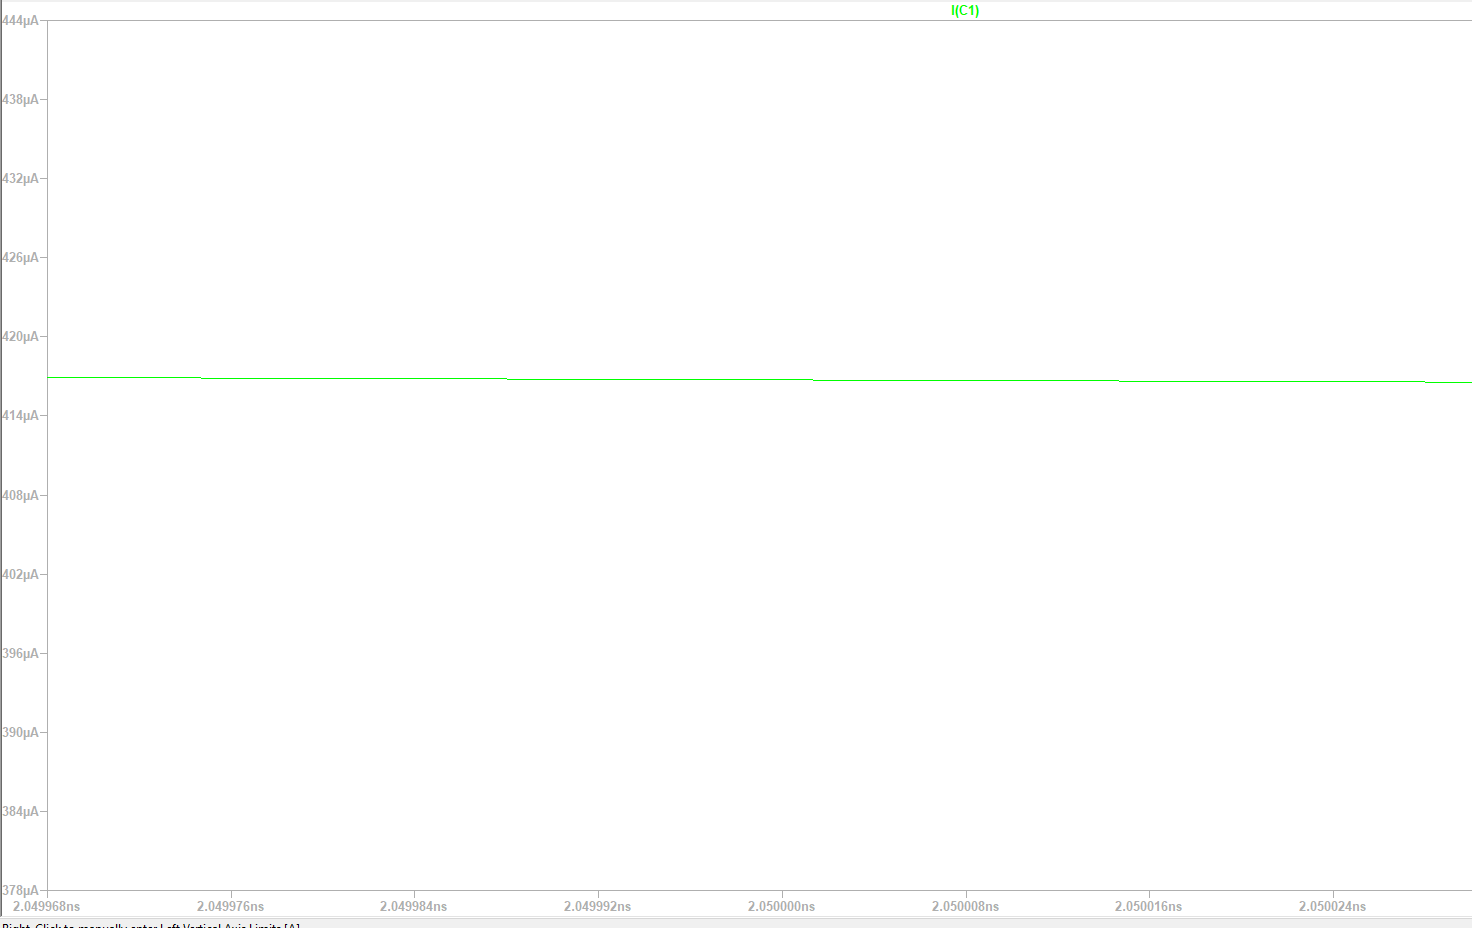
\includegraphics[scale=0.4]{CurrentPoint.PNG}
    \end{center}

\newpage
\section{La simulation du circuit}
    \begin{center}
        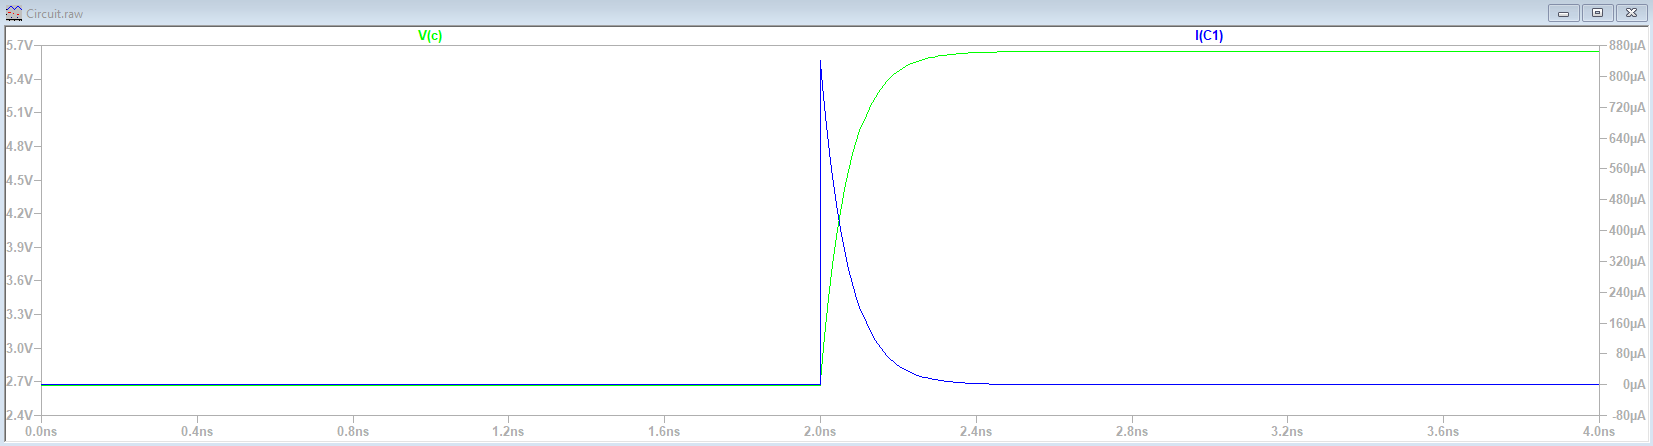
\includegraphics[scale=0.35]{Graph.PNG}
    \end{center}
    Ici on observe bien l'exemple d'un circuit transitoire où la tension et le courant évolue en fonction du temps
\section{Conclusion}
    Les résultats obtenu sont en adéquation avec ceux obtenu lors de la simulation LTspice XVII.
    \begin{itemize}
        \item On observe que la tension aux bornes de la capacité ainsi que le courant évolue en fonction du temps d'où le nom de régime transitoire.
    \end{itemize}
\end{document}
